%====================================================================================
\section{¿Qués es una serie estacionaria?}
%====================================================================================
\begin{frame}{¿Qués es una serie estacionaria?}
	\begin{itemize}
		\item  La autocovarianza es importante porque proporciona un resumen básico de la dinámica de una serie .
		\item Obsérvese que la función de autocovarianza es simétrica:
			$$\gamma_k = \gamma_{-k}$$
		\item La simetría refleja el hecho que la autocovarianza sólo depende del desplazamiento, no importa si avanzamos y retrocedemos.
		\item También obsérvese que:
			$$\gamma_k = cov(Z_t,Z_t)=var(Z_t)$$
	\end{itemize}
\end{frame}
%---------------------------------------------------
\begin{frame}{¿Qués es una serie estacionaria?}
	\begin{itemize}
		\item  Recuerda también que la correlación entre dos variables aleatorias $x$, $y$ se define como:
			$$corr(x,y) = \frac{cov(x,y)}{\sigma_x \sigma_y}$$
		\item En vista de una mejor interpretación se prefiere la correlación y no la covarianza. Es decir se trabaja con la función de autocorrelación ? y no con la de autocovarianza $\gamma$:
			$$\rho_k = \frac{cov(Z_t, Z_{t-k})}{\sqrt{var(Z_t)}\sqrt{var(Z_{t-k})}} = \frac{\gamma_k}{\sqrt{\gamma_0}\sqrt{\gamma_0}} = \frac{\gamma_k}{\gamma_0}$$
	\end{itemize}
\end{frame}
%---------------------------------------------------
\begin{frame}{¿Qués es una serie estacionaria?}
	\begin{itemize}
		\item Otro concepto que vamos a emplear es el de la \textbf{autocorrelación parcial}.
		\item Las autocorrelaciones parciales miden la asociación entre $Z_t$ y $Z_{t-k}$ después de controlar los efectos intermedios $Z_t-1, \ldots Z_{t-k+1}$
		\item En términos prácticos la autocorrelación parcial es el coeficiente de $Z_{t-k}$ en una regresión lineal de $Z_t$ en $Z_t-1, \ldots Z_{t-k}$
		\item La herramienta gráfica que relaciona tanto la autocovarianza como la autocorrelación con el número de rezagos se conoce como \textbf{correlograma}
	\end{itemize}
\end{frame}
%---------------------------------------------------
\begin{frame}{Correlograma}
	\centering
		\begin{figure}
			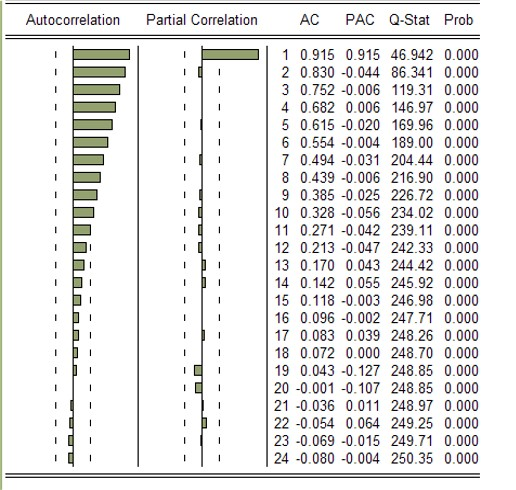
\includegraphics[width = 0.75\linewidth]{fig/figure5.jpg}
		\end{figure}
\end{frame}